\section{\seccolorgraphs}
\label{sec_color_graphs}

In many logistical applications of graph theory, the problem can be translated into a question about coloring graphs.  Examples of such applications include\footnote{source: wikipedia, graph coloring} scheduling (events or tasks), resource allocation  (such as assigning computer registers), and physical arrangements (such as assigning seating). In this section, we introduce graph coloring, look at applications to scheduling, and consider the minimum number of colors needed for standard graphs.

%%%%%%%%%%%%%%%%%%%%%%%%
\newcommand{\subcolormaps}{Coloring Maps}
\subsection{\subcolormaps}
\label{sub_color_maps}

Another application of graph coloring is coloring regions of a map.  We begin with an activity.

\begin{act}[Map coloring]
\label{act_map_coloring}

There are two rules for coloring a map.
\begin{description}
\item[\quad Rule 1:] Each region gets a single color.
\item[\quad Rule 2:] Any two regions that share a common border (more than a point) must be different colors.
\end{description}

    \begin{actpart}
        \item \label{part_map_coloring} Following these rules, color the map in \Cref{fig_map_coloring} using the colors blue, green, red, and purple. 
        
            \begin{figure}[hbtp]
                \centering               
                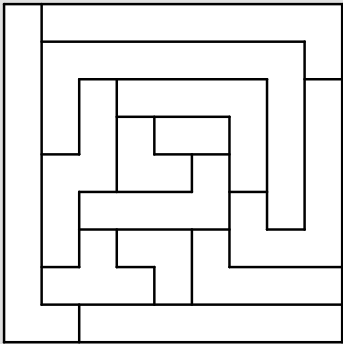
\includegraphics[scale=0.3]{Puzzles/Puzzle_Images/Four_color_map.png}
                \caption{A map to color.}
                \label{fig_map_coloring}
            \end{figure}
        
        You can use letters for the colors, such as \textbf{B} = blue, \textbf{G} = green, \textbf{R} = red, \textbf{P} = purple. You can color it by hand or go to the website: \url{https://www.geogebra.org/m/pjPgJdhV}
        (or Google search for ``Four Color Challenge''), color the map there, and capture a screenshot of your solution.

        \item Draw a rectangle and divide it into six regions to create a new map that can be colored using only two colors.  And show how to color it using \textbf{B} = blue and \textbf{G} = green.

        \item Draw a rectangle and divide it into six regions to create a new map that can be colored using three colors but not two colors.  Show how to color it using three colors: \textbf{B} = blue, \textbf{G} = green, and \textbf{R} = red and explain why it is impossible to color it using only two colors.

        \item In the map you colored in (\ref{part_map_coloring}), find a portion of the map with four regions where all four colors were needed.  Copy that portion of the map and show that four colors work using \textbf{B} = blue, \textbf{G} = green, \textbf{R} = red, \textbf{P} = purple.  Next, explain why it is impossible to color that portion of the map using only three colors.  Hint: if it is possible to color that portion of the map using only three colors, then you need to pick a different portion.
    \end{actpart}
\end{act}

We can model a map with a graph and rephrase our question about coloring a map into a question about coloring a graph.

\begin{exam}[Map coloring]
\label{exam_map_coloring}
~
    \begin{apart}
        \item Draw a graph with a vertex for each region of the map of midwest states shown in \Cref{fig_midwest_map} (in \Cref{sec_graph_models} \Cref{exer_midwest_MAP}).  Draw an edge between two vertices if the corresponding regions share an edge (more than a point).

            \begin{soln}
                We draw the map in \Cref{fig_graph_midwest}.             
            \end{soln}

            \begin{figure}[hbtp]
                \centering
                %Used in \Cref{sec_std_graphs}

\begin{tikzpicture}
    [scale =.5]
    \GraphInit[vstyle=Welsh]
    \SetGraphUnit{2}
    %\SetVertexNoLabel
    %%%%%%%
    \Vertex[LabelOut,Lpos=180,x=0,y=10]{ND}
    \Vertex[LabelOut,Lpos=45,x=3,y=9]{MN}

    \Vertex[LabelOut,Lpos=0,x=6,y=9]{WI}
    \Vertex[LabelOut,Lpos=180,x=0,y=8]{SD}
    \Vertex[LabelOut,Lpos=0,x=3,y=7]{IA}
    
    \Vertex[LabelOut,Lpos=180,x=0,y=6]{NE}

    \Vertex[LabelOut,Lpos=0,x=6,y=5]{IL}
    \Vertex[LabelOut,Lpos=-45,x=3,y=4]{MO}
    \Vertex[LabelOut,Lpos=180,x=0,y=4]{KS}
    \Vertex[LabelOut,Lpos=0,x=3,y=2]{AR}
    \Vertex[LabelOut,Lpos=180,x=0,y=2]{OK}
    \Vertex[LabelOut,Lpos=0,x=3,y=0]{LA}
    \Vertex[LabelOut,Lpos=180,x=0,y=0]{TX}

    \Edges(ND,SD,NE,KS,OK,TX)
    \Edges(MN,IA,MO,AR,LA)
    \Edges(WI,IL)
    \Edges(ND,MN,SD,IA,NE,MO,KS)
    \Edges(MO,OK,AR,TX,LA)
    \Edges(MN,WI,IA,IL,MO)
\end{tikzpicture}
                \caption{A map of midwest states.}
                \label{fig_graph_midwest}
            \end{figure}
        \item Rephrase the map coloring question as a question about the graph.
            \begin{soln}
                What is the smallest number of colors that we need in order to color the vertices of the graph in such a way that adjacent vertices are different colors?
            \end{soln}
    \end{apart}
\end{exam}

%%%%%%%%%%%%%%%%%%%%%%%%
\newcommand{\subchromatic}{Coloring Graphs}
\subsection{\subchromatic}
\label{sub_chromatic_number}

Let's formalize the idea of coloring the vertices of a graph.

\begin{defn}[Chromatic number]
\label{defn_chromatic_number}
~
    \begin{apart}
        \item A \vocab{(vertex) coloring} of a graph is an assignment of a color to each vertex in such a way that adjacent vertices have different colors. 
        \item A \vocab{$k$-coloring} of a graph is a vertex coloring using $k$ colors.  For example, the graph in \Cref{fig_schedule_alumni_colors} has a 3-coloring.
        \item A graph is \vocab{$k$-colorable} if there exists a coloring using $k$ or fewer colors.
        \item The \vocab{chromatic number} of a graph is the smallest number of colors needed to color the graph.  For example, the complete bipartite graph, $K_{6,3}$, shown in \Cref{fig_K6_again} has chromatic number two because it can be colored using two colors (black and white) and one color would not work because there are adjacent vertices. 
    \end{apart}
\end{defn}

Let's look at a few examples.

\begin{exam}[Chromatic number of complete graph and cycle]
\label{exam_chromatic_K5_C5}
    Determine the chromatic number $k$ of each graph by finding a $k$-coloring and then explaining why all $k$ colors are necessary.
        \begin{apart}
            \item The complete graph $K_5$.
                \begin{soln}
                    First, we can color each vertex its own color using five colors.  Since any pair of vertices in $K_5$ are adjacent, they must be different colors and so we cannot use fewer than five colors.  Thus, the chromatic number of $K_5$ is five.
                \end{soln}
                
            \item  The cycle $C_5$.
                \begin{soln}
                    If we try to color the vertices of $C_5$ using only two colors (gray and black), as shown in \Cref{fig_C5_3colored}, we run into a problem.  The fifth vertex cannot be gray (because it is adjacent to a vertex colored gray) and it cannot be black (because it is adjacent to a vertex colored black).  It must be a third color, say white.

                        \begin{figure}[hbtp]
                            \centering
                            %Used in \Cref{sec_std_graphs}.

% A 3-coloring of C_5
\begin{tikzpicture}
    [scale =.5]
    \GraphInit[vstyle=Welsh]
    \SetGraphUnit{2}
    \SetVertexNoLabel
    \Vertices{circle}{a,b,c,d,e}
    \Edges(a,b,c,d,e,a)

    % Coloring the Vertices        
        \AddVertexColor{black}{a,c}
        \AddVertexColor{gray}{b,e}
\end{tikzpicture}


                            \caption{Coloring the cycle $C_5$.}
                            \label{fig_C5_3colored}
                        \end{figure}
                    
                    Notice that \Cref{fig_C5_3colored} actually shows that three colors (gray, black, and white) work.  Thus, the chromatic number of $C_5$ is three.
                \end{soln}
        \end{apart}
\end{exam}

Let's try determining the chromatic number of graphs.

\begin{act}[Chromatic number of graphs]
\label{act_chromatic_number}
    To show the chromatic number of a graph is $k$, you should draw the graph, show how to color the vertices using $k$ colors, and then explain why fewer than $k$ colors cannot work.
    \begin{actpart}
        \item \label{part_chromatic_C5} Explain why the chromatic number of the cycle graph $C_4$ is two but the chromatic number of the cycle graph $C_5$ is three.

        \item \label{part_color_W5} Find the chromatic number of the wheel graph $W_5$.  Hint: use (\ref{part_chromatic_C5}).
        
        \item \label{part_chromatic_K4} What's the chromatic number of $K_4$?  Explain.

        \item \label{part_color_E} The graph $E$ drawn in \Cref{fig_elephant_nolabel}.  Find the chromatic number of $E$.  Hint: use the result of (\ref{part_chromatic_K4}).

            \begin{figure}[hbtp]
                \centering
                \input{Tikz/elephant_nolabel}
                \caption{The graph $E$.}
                \label{fig_elephant_nolabel}
            \end{figure}
    \end{actpart}
\end{act}

Let's look at \Cref{act_chromatic_number} (\ref{part_color_W5}) and (\ref{part_color_E}).

\begin{exam}[Chromatic number of complicated graphs]
\label{exam_chromatic_complicated}
~
    \begin{apart}
                
        \item Find the chromatic number of the wheel graph $W_5$. 
            \begin{soln}
                First, notice that the five outer vertices form a copy of $C_5$.  Since $C_5$ has chromatic number three, the outer vertices require at least three different colors. The hub vertex is adjacent to all five outer vertices, and so it must be yet another color.  Therefore, we need at least four colors to color the wheel $W_5$. 
                    
                Second, \Cref{fig_wheel5_4colored} shows a 4-coloring of the wheel $W_5$. Thus, the chromatic number of the wheel $W_5$ is four.
            \end{soln}

                \begin{figure}[hbtp]
                    \centering
                    %Used in \Cref{sec_std_graphs}.

\begin{tikzpicture}
    [scale =.5]
    \GraphInit[vstyle=Welsh]
    \SetGraphUnit{2}
    \SetVertexNoLabel
% W5
    \Vertices{circle}{a,b,c,d,e}
    \Vertex[x=0,y=0]{z}
    \Edges(a,b,c,d,e,a)
    \Edges(a,z,b)
    \Edges(c,z,d)
    \Edges(e,z)

% Coloring the Vertices        
        \AddVertexColor{black}{a,c}
        \AddVertexColor{gray}{b,e}
        \AddVertexColor{lightgray}{z}
\end{tikzpicture}
                    \caption{A 4-coloring of the wheel $W_5$.}
                    \label{fig_wheel5_4colored}
                \end{figure}
        \item Find the chromatic number of the graph $E$ drawn in \Cref{fig_elephant_nolabel}. 
            \begin{soln}
                First, notice that the center four vertices form a copy of $K_4$.  Since $K_4$ has chromatic number four, we know that those four vertices must be four different colors.  Therefore, we need at least four colors to color the entire graph $E$. 
                    
                Second, \Cref{fig_elephant_4colored} shows a 4-coloring of the graph. Thus, the chromatic number of $E$ is four.
            \end{soln}

                \begin{figure}[hbtp]
                    \centering
                    \input{Tikz/elephant_4colored}
                    \caption{A 4-coloring of the graph $E$.}
                    \label{fig_elephant_4colored}
                \end{figure}

    \end{apart}
\end{exam}

Coloring can be used to solve scheduling problems.

\begin{exam}[Scheduling alumni events]
\label{exam_scheduling_alumni}
There are three time slots for alumni events this Saturday:  late morning, early afternoon, or late afternoon. 
    \begin{bull}
        \item Alumni Office events:  Meet \& Greet (M), Campus Tours (C), and Alumni Panel (A).
        \item Theater Department events:  Poetry Slam (P), Screenplay Reading (R), and Viewing Student Films (V).
        \item Career Services events:  Speed Networking (N), Interviews (I), and Leadership Development Workshop (L). 
    \end{bull}
    Each organization can run only one of its events at a time.
    In addition, events A and V both want to use the theater and events M, P, and N all want to use the main conference hall, so those events need to be at different times. 
    \begin{apart}
        \item Draw a graph representing the situation where each event is a vertex and an edge connects two events if they cannot be scheduled in the same time block.
            \begin{soln}
                See \Cref{fig_schedule_alumni}.
                \begin{figure}
                    \centering                    
                    \input{Tikz/Sch_alum}
                    \caption{Graph for scheduling alumni events.}
                    \label{fig_schedule_alumni}
                \end{figure}
            \end{soln}

        \item \label{part_schedule_events} Is there a way to assign events times?  
            \begin{soln}
                Yes, one solution is M, R, and L in late morning; C, V, and N in early afternoon; and A, P, and I in late afternoon. 
            \end{soln}
        \item Color each vertex with a time that event could be scheduled using the key: black = late morning, gray = early afternoon, and white = late afternoon. 
            \begin{soln}
                See \Cref{fig_schedule_alumni_colors}.

                \begin{figure}[hbtp]
                    \centering
                    %Used in \Cref{sec_graph_models}.

\begin{tikzpicture}
    [scale =.4]
    \GraphInit[vstyle=Welsh]
    \SetGraphUnit{2}
    %\SetVertexNoLabel
% Vert
    % First column
        \Vertex[LabelOut,Lpos=90,x=0,y=4]{M}
        \Vertex[LabelOut,Lpos=180,x=0,y=2]{C}
        \Vertex[LabelOut,Lpos=-90,x=0,y=0]{A}
    % Second column
        \Vertex[LabelOut,Lpos=90,x=4,y=4]{P}
        \Vertex[LabelOut,Lpos=180,x=4,y=2]{R}
        \Vertex[LabelOut,Lpos=-90,x=4,y=0]{V}
    % Third column
        \Vertex[LabelOut,Lpos=90,x=8,y=4]{N}
        \Vertex[LabelOut,Lpos=180,x=8,y=2]{I}
        \Vertex[LabelOut,Lpos=-90,x=8,y=0]{L}
    % Straight Edges    
        \Edges(M,C,A) 
        \Edges(P,R,V) 
        \Edges(N,I,L) 
        \Edges(A,V)
        \Edges(M,P,N) %MN
    % Curved Edges
        \draw (M)  to [out=-45,in=45,in looseness=1.7] (A);
        \draw (P)  to [out=-45,in=45,in looseness=1.7] (V);
        \draw (N)  to [out=-45,in=45,in looseness=1.7] (L);
        \draw (M)  to [out=30,in=150,in looseness=1.7] (N);
    % Coloring the Vertices        
        \AddVertexColor{black}{M,R,L}
        \AddVertexColor{gray}{C,V,N}
\end{tikzpicture}
                    \caption{Graph for scheduling alumni events where colors represent event time.}
                    \label{fig_schedule_alumni_colors}
                \end{figure}
            \end{soln}
        \item Restate the question from (\ref{part_schedule_events}) in terms of the graph and colors.
            \begin{soln}
                Can we color the vertices of the graph using three colors so that adjacent vertices are different colors?
            \end{soln}        
    \end{apart}   
\end{exam}

%%%%%%%%%%%%%%%%%%%%%%%%
\newcommand{\subgraphconj}{Graph Conjectures}
\subsection{\subgraphconj}
\label{sub_graph_conj}

We have looked at several specific graphs and calculated quantities such as the number of vertices and edges, the degree sequence, and the chromatic number.  What about families of graphs?  Let's look at an example.

\begin{exam}[Graph conjectures for the complete graphs]
\label{exam_graph_conj_Ks}
    Consider the complete graphs $K_s$ for $s \ge 1$.  Conjecture the number of vertices and edges, the degree sequence, and the chromatic number of $K_s$. Some of your answers should involve $s$.  
        \begin{soln}
            By definition, $K_s$ has $s$ vertices.  Recall that $K_s$ models the number of handshakes in a group of $s$ people.  By \Cref{thm_hs}, the number of edges is $1+2+3+\ldots+(s-1) = \frac{s(s-1)}{2}$.  Alternatively, there is an edge for each pair of vertices. Thus, the number of edges is equal to the number of ways to select two out of $s$ vertices, which is $\binom{s}{2}$.

            Each vertex in $K_s$ is adjacent to each of the other $s-1$ vertices. Therefore, the degree sequence is
                $$\underbrace{s-1,s-1,s-1, \ldots, s-1}_{s \text{ times}}.$$

            We can color the vertices of $K_s$ with $s$ colors by assigning each vertex its own color.  Because each vertex is adjacent to every other vertex, no two vertices can be the same color.  Thus, all $s$ colors are necessary.  The chromatic number of $K_s$ is $s$.
        \end{soln}
\end{exam}

We summarize the number of edges of the complete graph $K_s$ for later reference.

\begin{thm}[Number of edges in the complete graphs]
\label{thm_size_Ks}
    For any positive integer $s$, the complete graph $K_s$ has 
        $$1+2+3+\ldots+(s-1) = \frac{s(s-1)}{2} = \binom{s}{2}$$
    edges.
\end{thm}

Try making conjectures about families of graphs.

\begin{act}[Graph conjectures]
\label{act_graph_conjectures}
~    
    \begin{actpart}
        \item Consider the star graphs $K_{1,t}$ for $t \ge 2$.  Conjecture the number of vertices and edges, the degree sequence, and the chromatic number of $K_{1,t}$. Some of your answers should involve $t$.  

        \item Consider the paths $P_s$ for $s \ge 2$. Conjecture the number of vertices and edges, the degree sequence, and the chromatic number of $P_s$. Some of your answers should involve $s$.

        \item Consider the cycles $C_s$ for $s \ge 3$. Conjecture the number of vertices and edges, the degree sequence, and the chromatic number of $C_s$. Some of your answers should involve $s$. 
    \end{actpart}
\end{act}

%%%%%%%%%%%%%%%%%%%%%%%%

\subsection{Exercises}

%%%%%%%%%%%%%%%%%%%%%%%%

\subsubsection*{Exercises for \Cref{sub_color_maps} \subcolormaps}

\begin{exer}[\exerP] % map coloring website]
\label{exer_map_coloring_website}
    Go to the website: \url{https://mathigon.org/course/graph-theory/map-colouring}
    to color more complicated maps.  Save screenshots of three puzzles that you attempted.  Were you able to solve all three?  If not, where did you get stuck?
\end{exer}

\begin{exer}[\exerP] % coloring northeast states]
\label{exer_color_northestUS} 
    Copy the map of the northeast states drawn in \Cref{fig_NE_states} and show how to 4-color the map. Note: Both parts of New York (NY) should be one color -- one part (Upstate New York) is labeled NY, the other part (NYC/Long Island) sits below Connecticut (CT)/Rhode Island (RI) and is long and skinny. 

    \begin{figure}[hbtp]
        \centering
        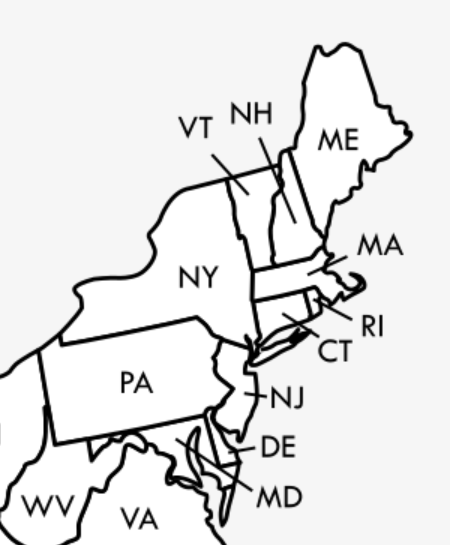
\includegraphics[scale=.3]{Puzzles/Puzzle_Images/NorthEastUStoColor.png}
        \caption{Map of the northeastern states.}
        \label{fig_NE_states}
    \end{figure}
\end{exer}

\begin{exer}[\exerU] % color the midwest map
\label{exer_midwest_color}
~    
    \begin{apart}
        \item Copy the map of midwest states drawn in \Cref{fig_midwest_map} (in \Cref{sec_graph_models} \Cref{exer_midwest_MAP}) and show how to color the map using three colors.  Note: We discussed this map in \Cref{exam_map_coloring}.
        \item Find a portion of the map where all three colors were needed.  Copy that portion of the map and explain why it is impossible to color that portion of the map using only two colors.  
    \end{apart}
\end{exer}

\begin{exer}[\exerR] % coloring maps
\label{exer_dyk_color_maps}
    Do you know \ldots
        \begin{exerpart}
            \item What the connection is between coloring a map and coloring a graph?
            \item How to draw a graph model of a map?
        \end{exerpart}
\end{exer}

\begin{exer}[\exerE] % the four color theorem]
~    Read the Quanta magazine article ``Only Computers Can Solve This Map-Coloring Problem'' and answer the following questions based on that article.
    \begin{exerpart}
        \item According to this article, the Four-Color Problem was introduced in a letter, which is a common way mathematics was communicated historically.  Who wrote the letter and to whom did they send it?
        \item What does the Four-Color Theorem say?
        \item When did the first proofs appear and who initially claimed to have proved it?
        \item How can the Four-Color Problem be restated in terms of graph theory?
        \item When did the final proof appear and who is credited with the final proof?
        \item Why did the presentation of the final proof receive only ``polite applause,'' according to mathematician Don Albers?
        \item The original, but flawed, proof has six ``special configurations.''  How many special configurations were considered in the final proof?
        \item What is allegedly in Paul Erd\"os's ``The Book''? 
    \end{exerpart} 
\end{exer}

%%%%%%%%%%%%%%%%%%%%%%%%

\subsubsection*{Exercises for \Cref{sub_chromatic_number} \subchromatic}

\begin{exer}[\exerP] % coloring standard graphs]
\label{exer_coloring_standard_graphs}
Draw each graph and color the vertices with the fewest possible colors.  No justification is necessary, but be sure that fewer colors would not work.    
        \begin{exerpart}
            \item The star $K_{1,6}$.           
            \item The path $P_6$.
            \item The cycle $C_6$.
            \item The wheel $W_6$.
            \item The ladder $L_{2\times3}$.
        \end{exerpart}
\end{exer}

\begin{exer}[\exerU] % chromatic number of classmates graph]
\label{exer_chromatic_number_classmates_graph}
~
    \begin{exerpart}
        \item Show how to 3-color the vertices of the classmates graph from \Cref{exam_classmates_graph} using red, blue, and green. 
        \item Explain why you need at least three colors to color the vertices of the classmates graph.
        \item What is the chromatic number of the classmates graph?  
    \end{exerpart}    
\end{exer}

\begin{exer} [\exerU] % coloring the complete graph $K_5$]
\label{exer_coloring_complete}
    Draw each graph and color the vertices with the fewest possible colors. Then explain why fewer colors would not work.  
    \begin{exerpart}
        \item The path $P_5$.
        \item The cycle $C_3$.
        \item The complete bipartite graph $K_{3,4}$.        
        \item The wheel $W_4$.
    \end{exerpart}
\end{exer}

\begin{exer} [\exerU] % prove chromatic number of a complicated graph]
\label{exer_color_complicated_graph}
   Consider the graph $H$ drawn in \Cref{fig_complicated_graph}.
        \begin{figure}[htbp]
            \centering
            %Appears in \Cref{sec_std_graphs}

\begin{tikzpicture}
[scale =.25, auto=left]
\GraphInit[vstyle=Welsh]
\SetGraphUnit{2}
\SetVertexNoLabel
\Vertex[LabelOut,Lpos=180,x=0,y=0]{$d$}
\Vertex[LabelOut,Lpos=180,x=0,y=8]{$a$}
\Vertex[LabelOut,Lpos=0,x=12,y=8]{$b$}
\Vertex[LabelOut,Lpos=0,x=12,y=0]{$c$}
%
\Vertex[LabelOut,Lpos=-90,x=4,y=2]{$w$}
\Vertex[LabelOut,Lpos=90,x=4,y=6]{$t$}
\Vertex[LabelOut,Lpos=-90,x=8,y=2]{$v$}
\Vertex[LabelOut,Lpos=90,x=8,y=6]{$u$}

\Edges($d$, $a$, $b$, $c$,$d$)
\Edges($t$,$u$, $v$, $w$, $t$)
\Edges($d$,$t$, $a$, $w$, $d$)
\Edges($b$,$v$, $c$, $u$, $b$)
\end{tikzpicture} 
            \caption{The graph $H$ from \Cref{exer_color_complicated_graph}.}
            \label{fig_complicated_graph}
        \end{figure}
    \begin{exerpart}
        \item \label{part_4coloring} Copy $H$ and show a 4-coloring of $H$.
        \item \label{part_4colors_suffice} Find a subgraph (portion) of $H$ that needs at least 4 colors.
        \item What can we conclude from (\ref{part_4coloring}) and (\ref{part_4colors_suffice})?
    \end{exerpart}   
\end{exer}

\begin{exer}[\exerU] % scheduling meetings]
\label{exer_schedule_meetings}
    There are seven people and seven committees.  Each person is on several committees, as described by \Cref{table_committee_members}.  There are four standard meeting times: 8-9:30 AM, 10-11:30 AM, 2-3:30 PM, and 4-5:30 PM.  We would like to schedule meeting times for the committees in such a way that we avoid having two meetings at the same time if any person is a member of both committees.  Is there a way to do it?

    \begin{table}[ht]
        \centering
        \begin{tabular} {c |c |c |c |c |c |c |c}
            Person on Cmte?&  Cmte 1 & Cmte 2 & Cmte 3 & Cmte 4 & Cmte 5 & Cmte 6 & Cmte 7 \\ \hline
            Alejandro & $\checkmark$ & $\checkmark$ & &&&& \\ \hline
            Bjorn & $\checkmark$ &  &$\checkmark$ &$\checkmark$&&& \\ \hline
            Cassie &  & $\checkmark$ & &&$\checkmark$&& \\ \hline
            Denise & $\checkmark$ &  & &&&$\checkmark$&$\checkmark$ \\ \hline
            Ebrahim & & & && $\checkmark$&&$\checkmark$  \\ \hline
            Fiona &  & $\checkmark$ & &$\checkmark$&&& \\ \hline
            Gloria  &  & &$\checkmark$ &$\checkmark$&&$\checkmark$& \\ 
        \end{tabular}
        \caption{Committee (cmte) members for \Cref{exer_schedule_meetings}.}
        \label{table_committee_members}
    \end{table}
    \begin{exerpart}
        \item Draw a graph to represent the situation where each committee is a vertex.  What should the edges represent?
        \item \label{part_schedule_meetings_color} Is there a way to assign meeting times?  If so, color each vertex with a time it could meet using the key: red is 8-9:30 AM, blue is 10-11:30 AM, green is 2-3:30 PM, and orange is 4-5:30 PM.  
        \item Restate the question from (\ref{part_schedule_meetings_color}) in terms of the graph and colors.
    \end{exerpart}
\end{exer}

\begin{exer}[\exerU] % chromatic number inequalities]
\label{exer_chr_ineq}
    What can we say about the chromatic number $k$ of a graph $G$ if \ldots?  Your answer should be a conjecture in the form of an equation or inequality involving $k$.
        \begin{exerpart}
            \item $G$ contains a copy of $K_5$.
            \item $G$ can be 5-colored.
        \end{exerpart}
\end{exer}

\begin{exer}[\exerR] % coloring graphs
\label{exer_dyk_color_graphs}
    Do you know \ldots
        \begin{exerpart}
            \item What a coloring of a graph is?
            \item What the chromatic number of a graph is?
            \item Which two things we need to check to determine the chromatic number of a graph?
            \item How to model a scheduling problem as a graph-coloring problem? 
        \end{exerpart}
\end{exer}

\begin{exer}[\exerE] % graph coloring algorithm
\label{exer_graph_color_algorithm}
    Here is an algorithm to 4-color the vertices of graph $G$ when the maximum degree of any vertex in $G$ is three.  
        \begin{enumerate}
            \item Assign each color a number: red (1), blue (2), green (3), and orange (4).  Label the vertices $v_1$, $v_2$, \ldots, $v_n$.  Color the vertex $v_1$ red (1). 
            \item Go to the next vertex and color it the smallest number color that is available, keeping in mind that the vertex cannot be colored the same as any adjacent vertex. Repeat this step until $v_n$ is colored.
        \end{enumerate}
     
        \begin{exerpart}
            \item Apply this process to color the graph shown in \Cref{fig_ladder_cross_color}.
                \begin{figure}[hbtp]
                    \centering
                    %Used in \Cref{sec_std_graphs}.

\begin{tikzpicture}
[scale =.55, auto=left]
\GraphInit[vstyle=Welsh]
\SetGraphUnit{1.6}
%\SetVertexNoLabel
\Vertices{circle}{$v_3$,$v_2$,$v_1$,$v_8$,$v_7$,$v_6$,$v_5$,$v_4$}
\Edges($v_1$,$v_2$,$v_3$,$v_4$,$v_5$,$v_6$,$v_7$,$v_8$,$v_1$)
\Edges($v_1$,$v_6$)
\Edges($v_2$,$v_5$)
\Edges($v_3$,$v_7$)
\Edges($v_4$,$v_8$)
\end{tikzpicture}
                    \caption{Use an algorithm to color the vertices of this graph}.
                    \label{fig_ladder_cross_color}
                \end{figure}
        
            \item Now consider a general graph $G$ where the maximum degree of any vertex is three. Explain why there will always be a color available in Step 2 of the algorithm.  Hint: Each vertex has degree three.
            \item What have we proved about the chromatic number of $G$? Hint: Your answer should be an inequality.
        \end{exerpart}
\end{exer}

\begin{exer}[\exerE] % examples of graphs with given chromatic number]
\label{exer_examples_chromatic_number}
~
    \begin{exerpart}
        \item Give an example of a graph with chromatic number two that is not a complete bipartite graph, a cycle, a path, a ladder, or a grid.
        \item Give an example of a graph with chromatic number five that is not a complete graph.
        \item Give an example of a graph with at least two vertices but chromatic number one.
    \end{exerpart}
\end{exer}

%%%%%%%%%%%%%%%%%%%%%%%%

\subsubsection*{Exercises for \Cref{sub_graph_conj} \subgraphconj}

\begin{exer}[\exerP] % graph conjectures for complete bipartite graphs and ladders]
\label{exer_graph_conjecture_Kbst}
    Consider the complete bipartite graphs $K_{s,t}$ for $s,t \ge 1$. Conjecture the number of vertices and edges, the degree sequence, and the chromatic number of $K_{s,t}$. Some of your answers should involve $s$ or $t$.
\end{exer}

\begin{exer}[\exerU] % graph conjecture wheels
\label{exer_graph_conj_wheels}
    Consider the wheels $W_s$ for $s \ge 3$. Conjecture the number of vertices and edges, the degree sequence, and the chromatic number of $W_s$. Some of your answers should involve $s$.  
\end{exer}

\begin{exer}[\exerU] 
\label{exer_graph_conj_ladders}
    Consider the ladders $L_{2 \times t}$ for $t \ge 2$. Conjecture the number of vertices and edges, the degree sequence, and the chromatic number of $L_{2 \times t}$. Some of your answers should involve $t$.
\end{exer}

\begin{exer}[\exerR] % graph conjectures
\label{exer_dyk_graph_conj}
    Do you know \ldots
        \begin{exerpart}
            \item How many edges $K_s$ has?
            \item How to count the number of vertices, the number of edges, the degree sequence, and the chromatic number for a family of graphs (in terms of parameters such as $s$ or $t$)?
        \end{exerpart}
\end{exer}

\begin{exer}[\exerE] % grid graphs]
\label{exer_grid_graphs}
    For $s,t \ge 1$, the \vocab{grid graph} (or \vocab{lattice graph}) is denoted $L_{s\times t}$.  Its vertices are the point,s $(x,y)$, in the $xy$-plane where $x = 1, 2, \ldots, s$ and $y = 1, 2, \ldots, t$.  There is an edge connecting two points with the same $x$-coordinate when their $y$-coordinates differ by 1. Also, there is an edge connecting two points with the same $y$-coordinate when their $x$-coordinates differ by 1.  The ladder graphs are the special case where $s=2$.
    \begin{exerpart}
        \item \label{part_gridpoints} List the vertices of $L_{3 \times 4}$ and draw those points in the $xy$-plane.
        \item List the edges of $L_{3 \times 4}$ and add those edges to your points from (\ref{part_gridpoints}).
        \item How many vertices does the graph $L_{s \times t}$ have? Your answer should involve $s$ and $t$.
        \item How many edges does the graph $L_{s \times t}$ have? Your answer should involve $s$ and $t$.
    \end{exerpart}
\end{exer}

\begin{exer}[\exerE] % perfect binary trees]
\label{exer_perfect_binary_trees}  
    \Cref{fig_perfect_binary_trees} shows drawings of perfect binary trees $B_1$, $B_2$, and $B_3$.
    
        \begin{figure} [hbtp]
            \centering
            %Appears in \Cref{sec_graph_models}

% B_1
\begin{tikzpicture}
[scale =.45, auto=left]
\GraphInit[vstyle=Welsh]
\SetGraphUnit{2}
\SetVertexNoLabel
% Root
\Vertex[x=3,y=4]{0}
% Children
\Vertex[x=2,y=2]{00}
\Vertex[x=4,y=2]{01}
% Edges
\Edges(0,00)
\Edges(0,01)
\end{tikzpicture}
\hspace{.35in} %%%%%%%%%
% B_2
\begin{tikzpicture}
[scale =.45, auto=left]
\GraphInit[vstyle=Welsh]
\SetGraphUnit{2}
\SetVertexNoLabel
% Root
\Vertex[x=3,y=4]{0}
% Children
\Vertex[x=1,y=2]{00}
\Vertex[x=5,y=2]{01}
% Grandchildren
\Vertex[x=0,y=0]{000}
\Vertex[x=2,y=0]{001}
\Vertex[x=4,y=0]{010}
\Vertex[x=6,y=0]{011}
% Edges
\Edges(0,00)
\Edges(0,01)
\Edges(00,000)
\Edges(00,001)
\Edges(01,010)
\Edges(01,011)
\end{tikzpicture} 
\hspace{.35in} %%%%%%%%%
% B_3
\begin{tikzpicture}
[scale =.45, auto=left]
\GraphInit[vstyle=Welsh]
\SetGraphUnit{2}
\SetVertexNoLabel
% Root
\Vertex[x=7,y=6]{0}
% Children
\Vertex[x=3.5,y=4]{00}
\Vertex[x=10.5,y=4]{01}
% Grandchildren
\Vertex[x=2,y=2]{000}
\Vertex[x=5,y=2]{001}
\Vertex[x=9,y=2]{010}
\Vertex[x=12,y=2]{011}
% And their kids
\Vertex[x=0.5,y=0]{0000}
\Vertex[x=2.5,y=0]{0001}
\Vertex[x=4,y=0]{0010}
\Vertex[x=6,y=0]{0011}
\Vertex[x=8,y=0]{0100}
\Vertex[x=10,y=0]{0101}
\Vertex[x=11.5,y=0]{0110}
\Vertex[x=13.5,y=0]{0111}
% Edges
\Edges(0,00)
\Edges(0,01)
\Edges(00,000)
\Edges(00,001)
\Edges(01,010)
\Edges(01,011)
\Edges(000,0000)
\Edges(000,0001)
\Edges(001,0010)
\Edges(001,0011)
\Edges(010,0100)
\Edges(010,0101)
\Edges(011,0110)
\Edges(011,0111)
\end{tikzpicture} 
            \caption{The perfect binary trees $B_1$, $B_2$, and $B_3$.}
            \label{fig_perfect_binary_trees}
        \end{figure}
        
    The tree $B_1$ has a \vocab{root} vertex at the top. The root vertex is adjacent to two \vocab{child} vertices drawn below. The tree $B_2$ starts with the tree $B_1$ and then, for each end vertex, draws two new adjacent child vertices below. These new vertices are \vocab{grandchildren} of the root.  The tree $B_3$ starts with $B_2$ and then, for each end vertex, draws two new adjacent child vertices below. These new vertices are \vocab{great-grandchildren} of the root.  This pattern continues to give a family of \vocab{perfect binary trees}, denoted $B_s$ for $s\ge 1$.
    \begin{exerpart}
        \item \label{part_perfect_binary_tree_verts} In the perfect binary tree $B_3$, count the number of children, the number of grandchildren, and the number of great-grandchildren of the root.  Use these numbers to find the number of vertices in $B_3$. Hint: don't forget the root.
        \item Draw the perfect binary tree $B_4$.
        \item Conjecture the number of \vocab{leaves}\footnote{In a natural tree the root is at the bottom and the leaves are at the top.  Graph trees are upside down.} (end vertices) in $B_s$.
        \item How many vertices does $B_s$ have?  Hint: add up the generations as in (\ref{part_perfect_binary_tree_verts}).
        \item How many edges does $B_s$ have? Explain. 
        \item What are the degrees of the vertices in $B_s$ and how many vertices of each degree are there?  Hint: The root and the leaves have degrees that are from the middle vertices.
    \end{exerpart}
\end{exer}

\begin{exer}[\exerE] % Number of edges in complement
\label{exer_size_graph_comp}
~
    \begin{exerpart}
        \item Draw the cycle $C_5$. Then, using a different colored pen, add the edges of the complement $\overline{C_5}$ to your graph. What is the resulting graph?
        \item Draw the path $P_5$. Then, using a different colored pen, add the edges of the complement $\overline{P_5}$ to your graph. What is the resulting graph?  It might look a little different than usual.
        \item If we draw a graph $G$ that has five vertices and then, using a different colored pen, we add the edges of the complement $\overline{G}$ to the graph, what is the resulting graph?  Explain.
        \item If $G$ is any graph with five vertices and $m$ edges, how many edges does the complement $\overline{G}$ have?
        \item Generalize: if $G$ is any graph with $s$ vertices and $m$ edges, how many edges does the complement $\overline{G}$ have?  Hint: \Cref{thm_size_Ks} is useful.   
    \end{exerpart}
\end{exer}

%%%%%%%%%%%%%%%%%%%%%%%%%%%
\subsection{\answers}
%%%%%%%%%%%%%%%%%%%%%%%

\subsubsection{\answers for \Cref{sub_color_maps} \subcolormaps}

\subsubsection*{\Cref{exer_map_coloring_website} \answers}
Note: You do not need to submit the screenshots.

\subsubsection*{\Cref{exer_midwest_color} \answers}
\begin{apart}
    \item Hint: Start with ND: red, SD: blue, MN: red.  Then, continue with states whose color must follow.  For example, Iowa (IA) must be green.  Continue.
    \item Hint: Explain why the region formed by ND, SD, and MN needs three colors.
\end{apart}


%%%%%%%%%%%%%%%%%%%%%%%%%%%

\subsubsection{\answers for \Cref{sub_chromatic_number} \subchromatic}

\subsubsection*{\Cref{exer_coloring_standard_graphs} \answers}
\begin{apart}
    \item Hint: Draw the usual star with black and white vertices.
    \item Hint: Two colors work.
    \item Hint: Two colors work.
    \item See \Cref{fig_wheel6_3colored}.

                    \begin{figure}[hbtp]
                    \centering
                    %Used in \Cref{sec_std_graphs}.

\begin{tikzpicture}
    [scale =.5]
    \GraphInit[vstyle=Welsh]
    \SetGraphUnit{2}
    \SetVertexNoLabel
% W6
    \Vertices{circle}{a,b,c,d,e,f}
    \Vertex[x=0,y=0]{z}
    \Edges(a,b,c,d,e,f,a)
    \Edges(a,z,b)
    \Edges(c,z,d)
    \Edges(e,z,f)

% Coloring the Vertices        
        \AddVertexColor{black}{a,c,e}
        \AddVertexColor{gray}{b,d,f}
\end{tikzpicture}
                    \caption{A 3-coloring of the wheel $W_6$.}
                    \label{fig_wheel6_3colored}
                \end{figure}
        \item Hint: Two colors work.
\end{apart}



\subsubsection*{\Cref{exer_color_complicated_graph} \answers}
\begin{apart}
    \item Hint: Verify that you have colored all the vertices and that any pair of adjacent vertices is different colors.
    \item Hint: Look for complete subgraphs.
    \item Hint: (a) tells us the chromatic number is at most four and (b) tells us the chromatic number is at least four.
\end{apart}

\subsubsection*{\Cref{exer_schedule_meetings} \answers}
\begin{apart}
    \item Hint: An edge should indicate that the two committees have at least one member in common, which means that that pair of committees cannot be scheduled at the same time.  The graph has seven vertices and 12 edges.
    \item Hint: yes
    \item Hint: Can we 4-color the graph?
\end{apart}

\subsubsection*{\Cref{exer_chr_ineq} \answers}
    \begin{apart}
        \item Hint: $K_5$ needs 5 colors, so $G$ needs 5 colors or maybe more colors.
        \item Hint: Maybe $G$ can be colored using fewer than 5 colors if we try again.
    \end{apart}

\subsubsection*{\Cref{exer_graph_color_algorithm} \answers}
\begin{apart}
    \item Hint: Color $v_1$ red, $v_2$ blue, $v_3$ red, \ldots
    \item Hint: When we get to a new vertex to color, how many colors are already used by its neighbors?  Explain why there is always at least one of the four colors available to color the new vertex?
    \item Hint: We have found a 4-coloring of the graph.  What does that tell us about the chromatic number?
\end{apart}

\subsubsection*{\Cref{exer_examples_chromatic_number} \answers}
There are many correct answers to each part.  The hints describe how to build one such example.
    \begin{apart}
        \item Hint: There are many correct answers.  Try starting with the star $K_{1,3}$ which is a complete bipartite graph, but then add more vertices and connect them with an edge to the leaves in $K_{1,3}$.
        \item Hint: Start with $K_5$ and add more to it, making sure you can still 5-color the graph.
        \item Hint: The graph does not have to be connected. (And it cannot be connected.)
    \end{apart}
%%%%%%%%%%%%%%%%%%%%%%%%%%%

\subsubsection{\answers for \Cref{sub_graph_conj} \subgraphconj}

\subsubsection*{\Cref{exer_graph_conjecture_Kbst} \answers}
    Hint: There are $s+t$ vertices, \underline{\quad~} edges, the degree sequence is $$\underbrace{t,t,\ldots, t}_{s \text{ times}}\underbrace{s,s,\ldots, s}_{t \text{ times}}$$
    (perhaps in the other order), and the chromatic number is two.

\subsubsection*{\Cref{exer_graph_conj_wheels} \answers}
    Hint: There are $s+1$ vertices, there is exactly one vertex with degree $s$, and the chromatic number is three or four depending on whether $s$ is even or odd (be sure to say which is which).

\subsubsection*{\Cref{exer_graph_conj_ladders} \answers}
    Hint: There are four vertices of degree two, and the rest have degree three. One way to count edges is to add the number of horizontal edges in the first row, the number of horizontal edges in the second row, and the number of vertical rungs.

    \begin{figure}[hbtp]
        \centering
        %Used in \Cref{sec_color_graphs}

\begin{tikzpicture}
    [scale =.5]
    \GraphInit[vstyle=Welsh]
    \SetGraphUnit{2}
        \SetVertexNoLabel
    % bottom row
    \Vertex[LabelOut,Lpos=90,x=0,y=0]{a1}
    \Vertex[
    LabelOut,Lpos=90,x=2,y=0]{b1} 
    \Vertex[LabelOut,Lpos=90,x=4,y=0]{c1}
    \Vertex[LabelOut,Lpos=90,x=6,y=0]{d1}    

    \Edges(a1,b1,c1,d1)
    % middle row
    \Vertex[LabelOut,Lpos=90,x=0,y=2]{a2}
    \Vertex[LabelOut,Lpos=90,x=2,y=2]{b2} 
    \Vertex[LabelOut,Lpos=90,x=4,y=2]{c2}
    \Vertex[LabelOut,Lpos=90,x=6,y=2]{d2}    

    \Edges(a2,b2,c2,d2)
    % top row
    \Vertex[LabelOut,Lpos=90,x=0,y=4]{a3}
    \Vertex[LabelOut,Lpos=90,x=2,y=4]{b3} 
    \Vertex[LabelOut,Lpos=90,x=4,y=4]{c3}
    \Vertex[LabelOut,Lpos=90,x=6,y=4]{d3}    
    
    \Edges(a3,b3,c3,d3)
    % vertical edges
    \Edges(a1,a2,a3)
    \Edges(b1,b2,b3)
    \Edges(c1,c2,c3)
    \Edges(d1,d2,d3)
\end{tikzpicture}
        \caption{The grid graph $L_{3 \times 4}$.}
        \label{fig_grid_3x4}
    \end{figure}
    
\subsubsection*{\Cref{exer_grid_graphs} \answers}

    \begin{apart}
        \item Hint: There are 12 vertices.
        \item Hint: The graph is drawn in \Cref{fig_grid_3x4}
        \item Hint: Multiply
        \item Hint: Count the number of vertical edges.  Then count the number of horizontal edges.  Then add your answers.
    \end{apart}


